In Chapter~\ref{ch:source-coding}, we saw how to encode a source such that it can be stored or sent over some channel, and decoded at a later point in time. We assumed that the channel used to send the encoded information was perfect, meaning that no information got altered or lost while being sent over the channel. In this chapter, we consider a different setting, where the channel possibly contains some \term{noise}, that may convert the channel input $x$ to some potentually different value $y$:

\begin{figure}[h]
\begin{center}
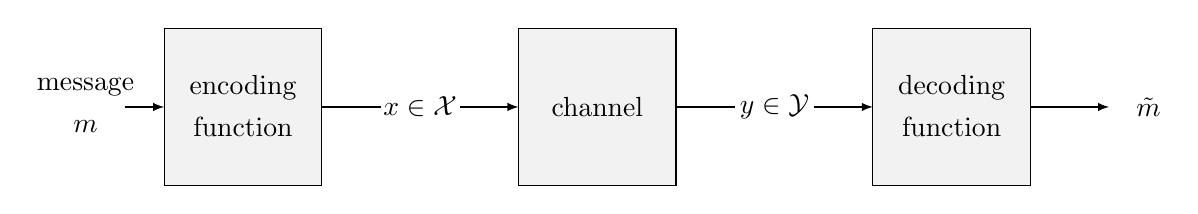
\begin{tikzpicture}
%\draw[fill=black!5] (0,0) rectangle (2,2);
%\node at (1,1.25) {$P_X$};
%\node at (1,0.75) {(source)};


%\draw[-latex] (2,1) -- (5,1);
%\draw[fill=white,draw=none] (2.5,0) rectangle (4.5,2);
%\node at (3.5,1.5) {$x$, with};
%\node at (3.5,1) {probability};
%\node at (3.5,0.5) {$P_X(x)$};
\node at (0,1.25) {message};
\node at (0,0.75) {$m$};
\draw[-latex] (0.5,1) -- (1,1);

\draw[fill=black!5] (1,0) rectangle (3,2);
\node at (2,1.25) {encoding};
\node at (2,0.75) {function};

\draw[-latex] (3,1) -- (5.5,1);
\fill[white] (3.75,0) rectangle (4.75,2);
\node at (4.25,1) {$x \in \mathcal{X}$};

\draw[fill=black!5] (5.5,0) rectangle (7.5,2);
\node at (6.5,1) {channel};

\draw[-latex] (7.5,1) -- (10,1);
\draw[fill=white,draw=none] (8.25,0) rectangle (9.25,2);
\node at (8.75,1) {$y \in \mathcal{Y}$};

\draw[fill=black!5] (10,0) rectangle (12,2);
\node at (11,1.25) {decoding};
\node at (11,0.75) {function};

\draw[-latex] (12,1) -- (13,1);
\node at (13.5,1) {$\tilde{m}$};
\end{tikzpicture}
\end{center}
\end{figure}
The goal is to design encoding and decoding functions that can resist this noise, so that the recovered message $\tilde{m}$ is as close as possible to the original message $m$. The question is how short (efficient) such codes can be while still providing resistance to noise.

\section{Channels}\label{sec:noisy-channel}
In this section, the notion of `channel' will me made more precise, and different types of channels are considered.

\begin{definition}[Discrete channel]
A (discrete) channel is a tuple $(\mathcal{X}, P_{Y|X}, \mathcal{Y})$ such that $\mathcal{X}$ and $\mathcal{Y}$ are finite, and $P_{Y|X} : \mathcal{Y} \to [0,1]$ is a probability distribution. $\mathcal{X}$ represents the set of possible inputs, $\mathcal{Y}$ the set of possible outputs, and $P_{Y|X}(y|x)$ is the probability of receiving output $y$ given an input $x$.
\end{definition}
Note that if we give a distribution $P_X$ for the set $\mathcal{X}$, this immediately determines a distribution $P_Y$ for $\mathcal{Y}$ by marginalization.

The above is a definition for \term{memoryless} channels, because the probability distribution of the output depends only on the (last) input. If the channel is used repeatedly, the distribution does not change dependent on previous inputs and outputs.

\begin{example}[Binary symmetric channel (BSC)]\label{example:binary-symmetric-channel}
Define the binary symmetric channel with parameter $f \in [0,1/2]$ by $\mathcal{X} = \mathcal{Y} = \set{0,1}$ and
\begin{align*}
P_{Y|X}(0|0) &= P_{Y|X}(1|1) = 1-f,\\
P_{Y|X}(0|1) &= P_{Y|X}(1|0) = f.\\
\end{align*}
With probability $f$, the input is flipped, and with probability $1-f$, it remains unaffected. This channel can be represented visually as
\begin{center}
\begin{tikzpicture}
\fill[ocre] (0,0) circle (1mm);
\fill[ocre] (0,2) circle (1mm);
\fill[ocre] (5,0) circle (1mm);
\fill[ocre] (5,2) circle (1mm);
\node at (-2,1) {(in)};
\node at (7,1) {(out)};
\node[anchor=east] at (-0.2,0) {1};
\node[anchor=east] at (-0.2,2) {0};
\node[anchor=west] at (5.2,0) {1};
\node[anchor=west] at (5.2,2) {0};

\draw (0.2,0) -- (4.8,0);
\draw (0.2,2) -- (4.8,2);
\draw (0.2,0) -- (4.8,2);
\draw (0.2,2) -- (4.8,0);

\fill[black!5] (2,0.25) rectangle (3,-0.25);
\fill[black!5] (2,2.25) rectangle (3,1.75);
\node at (2.5,-0.1) {$1-f$};
\node at (2.5,2.1) {$1-f$};

\fill[black!5] (1.25,0.25) rectangle (1.75,0.75);
\fill[black!5] (1.25,1.75) rectangle (1.75,1.25);
\node at (1.5,0.5) {$f$};
\node at (1.5,1.5) {$f$};
\end{tikzpicture}
\end{center} 
\end{example}
\begin{exercise}
Verify that, up to relabeling of the outputs in $\mathcal{Y}$, a BSC with parameter $f \in [1/2,1]$ is equivalent to a BSC with parameter $1-f$.
\end{exercise}
If we use the same channel $n$ times, without allowing the receiver to give feedback to the sender in between uses, this can be regarded as the channel $(\mathcal{X}^n, P_{Y^n|X^n}, \mathcal{Y}^n)$ where
\begin{align}
P_{Y^n|X^n}(\vec{y}|\vec{x}) = \prod_{i=1}^n P_{Y|X}(y_i|x_i),
\end{align}
because the channel is memoryless.

\begin{example}
If we send 00110 over the binary symmetric channel from Example~\ref{example:binary-symmetric-channel}, we receive the output 01111 with probability
\[
(1-f) \cdot f \cdot (1-f) \cdot (1-f) \cdot f = (1-f)^3f^2.
\]
In general, if a binary symmetric channel with noise parameter $f$ is used $n$ times, the probability of observing $k$ bit flips is
\[
{n \choose k} f^{k} (1-f)^{n-k}.
\]
\end{example}

\begin{example}
A binary symmetric channel (see Example~\ref{example:binary-symmetric-channel}) with parameter 0.1 is used to send $10^4$ bits. The bit flips that result from the channel use are distributed according to the binomial($10^4,0.1$) distribution: on expectation, $10^4 \cdot 0.1 = 1000$ bits are flipped, and the variance is $10^4 \cdot 0.1 \cdot 0.9 = 900$. Hence the \href{https://en.wikipedia.org/wiki/Standard_deviation}{standard deviation} is $\sqrt{900} = 30$. With probability 99.7$\%$, the number of bits that are flipped stays within three standard deviations of the mean, i.e. between 910 and 1090 bits are flipped with very high probability.
\end{example}

\begin{definition}[Deterministic channel]
A channel is deterministic if $H(Y|X) = 0$. In other words,
\[
\forall x \in \mathcal{X}\  \exists y \in \mathcal{Y}: P_{Y|X}(y|x) = 1.
\]
\end{definition}
\begin{definition}[Lossless channel]
A channel is lossless (or \term{ideal}) if $H(X|Y) = 0$. In other words,
\[
\forall y \in \mathcal{Y}\  \exists! x \in \mathcal{X}: P_{Y|X}(y|x) > 0.
\]
(the notation $\exists!x$ means that there exists \emph{exactly} one such $x$.)
\end{definition}
In a deterministic channel, the output is completely determined by the input, whereas in a lossless channel, the input is completely determined by the output.
A \term{noiseless} channel is a channel that is both deterministic and lossless.

\begin{example}\label{example:channel}
Consider the following channels. The connecting lines represent non-zero probabilities, but probabilities and inputs/outputs are not further specified (inputs are on the left, outputs on the right):\\
\begin{tikzpicture}
\fill[ocre] (0,0) circle (1mm);
\fill[ocre] (0,1) circle (1mm);
\fill[ocre] (2,0) circle (1mm);
\fill[ocre] (2,1) circle (1mm);
\draw (0.2,0) -- (1.8,0);
\draw (0.2,1) -- (1.8,1);

\fill[ocre] (4,1) circle (1mm);
\fill[ocre] (4,2) circle (1mm);
\fill[ocre] (6,0) circle (1mm);
\fill[ocre] (6,1) circle (1mm);
\fill[ocre] (6,2) circle (1mm);
\draw (4.2,1) -- (5.8,0);
\draw (4.2,1) -- (5.8,1);
\draw (4.2,2) -- (5.8,2);

\fill[ocre] (8,1) circle (1mm);
\fill[ocre] (8,2) circle (1mm);
\fill[ocre] (8,0) circle (1mm);
\fill[ocre] (10,1) circle (1mm);
\draw (8.2,0) -- (9.8,1);
\draw (8.2,1) -- (9.8,1);
\draw (8.2,2) -- (9.8,1);

\fill[ocre] (12,0) circle (1mm);
\fill[ocre] (12,1) circle (1mm);
\fill[ocre] (14,0) circle (1mm);
\fill[ocre] (14,1) circle (1mm);
\draw (12.2,0) -- (13.8,0);
\draw (12.2,1) -- (13.8,0);
\draw (12.2,0) -- (13.8,1);
\draw (12.2,1) -- (13.8,1);

\node at (1,-1) {(a)};
\node at (5,-1) {(b)};
\node at (9,-1) {(c)};
\node at (13,-1) {(d)};
\end{tikzpicture}
\\Channel (a) is both deterministic and lossless (and is therefore called a noiseless channel). Channel (b) is lossless but not deterministic, channel (c) is deterministic but not lossless, and channel (d) (the noisy binary channel) is neither.
\end{example}

For a given channel, we can ask ourselves: how much information could, in theory, be transmitted through a channel? In other words, what is its capacity?

\begin{definition}[Channel capacity]
Let $(\mathcal{X}, P_{Y|X}, \mathcal{Y})$ be a channel. Its capacity $C$ is defined as
\[
C := \max_{P_X} I(X;Y).
\]
\end{definition}

\begin{exercise}
What is the capacity of an ideal channel? What is the maximizing distribution $P_X$?
\end{exercise}


\section{Codes}
In order to get as much information through a channel as possible, we can try to find an optimal encoding of the message.

\begin{definition}[Code]\label{def:code}
Let $M, n \in \mathbb{N}$. An $(M,n)$-code for the channel $(\mathcal{X},P_{Y|X},\mathcal{Y})$ consists of
\begin{itemize}
\item An index set $[M] = \{1, ..., M\}$ representing the set of possible messages.
\item A (possibly probabilistic) encoding function $\mathtt{enc} :[M] \to \mathcal{X}^n$. This encoding function should be injective. $n$ represents the number of channel uses we need to send a single message.
\item A deterministic decoding function $\mathtt{dec} : \mathcal{Y}^n \to [M]$.
The set of all codewords, $\{\mathtt{enc}(1), ..., \mathtt{enc}(M)\}$ is called the \term{codebook}.
\end{itemize}
\end{definition}

\noindent The number of bits of information that are transmitted per channel use is captured by the following notion:

\begin{definition}[Rate]
The rate of an $(M,n)$-code is defined as
\[
R := \frac{\log M}{n}.
\]
\end{definition}

Given a code for a specific channel, we can wonder what the probability is that an error occurs while transmitting a message. For a fixed message $m$, this probability is represented by the following quantity.

\begin{definition}[Probability of error]\label{def:probability-of-error}
Given an $(M,n)$ code for a channel $(\mathcal{X},P_{Y|X},\mathcal{Y})$, the probability of error $\lambda_m$ is the probability that the decoded output is not equal to the input message $m$. More formally,
\[
\lambda_m := P[\mathtt{dec}(Y^n) \neq m \mid X^n = \mathtt{enc}(m)].
\]
Given this quantity, the \term{maximal probability of error} is defined as 
\[\lambda^{(n)} := \max_{m \in [M]} \lambda_m.\]
Similarly, the \term{average probability of error} is defined as
\[
p_e^{(n)} := \frac{1}{M} \sum_{m=1}^M \lambda_m.
\]
\end{definition}

\subsection{Repetition codes}
A simple and intuitive code is the $n$-bit \term{repetition code} $R_n$: a single message bit is encoded by simply repeating the bit $n$ times. Decoding is done by `majority vote', that is, $\mathtt{dec}(y) = MAJ(y_1, ..., y_n)$, which is 1 if and only if more than half of the bits in $y$ are 1s.

\begin{example}[3-bit repetition code]
Consider the 3-bit repetition code $R_3$. It is a (2,3) code with codebook $\{000,111\}$. The rate of $R_3$ is $1/3$. The probability of error for the message $m = 0$, sent over a BSC with bit flip propability $f$, is
\begin{align*}
\lambda_0 &= P[\mathtt{dec}(Y^n) \neq 0 \mid X^n = 000]\\
&= P[Y^n = 011 \ \cup \ Y^n = 101 \ \cup \ Y^n = 110 \ \cup \ Y^n = 111 \mid X^n = 000]\\
&= 3f^2(1-f) + f^3.
\end{align*}
A similar calculation shows that $\lambda_1 = \lambda_0$. Hence, the maximal and average probability of error are equal to $\lambda_0$ as well.

As a concrete example, if $f = 0.1$, the 3-bit repetition code has an error probability of approximately 0.03. Hence, the 3-bit repetition code provides an error probability that is about three times lower ($3\%$ instead of $10\%$), at the expense of a rate that is a factor 3 worse than simply sending the messages through the channel without encoding.
\end{example}
In general, the $n$-bit repetition code is a $(2,n)$ code with the relatively low rate of $1/n$ and an average/maximal probability of error of
\[
\sum_{k=(n+1)/2}^n {n \choose k} f^k (1-f)^{n-k}
\]
when used on a binary symmetric channel with bit flip probability $f$.

\begin{example}[Application of the repetition code]
A company producing hard drives wants to make sure that the probability that a customer experiences a storage failure is at most $0.1\%$. The company has 1000 customers, who each want to store 10 GB of data for 10 years without experiencing a failure. That means that the probability of a single stored bit being stored incorrectly has to be at most
\[
\frac{1}{10 \cdot 8 \cdot 10^9} \cdot \frac{1}{10 \cdot 365} \cdot \frac{1}{1000} \cdot 0.001 \geq 10^{-20}
\]
in order to store 10 GB a day for 10 years on 1000 drives with total failure probability 0.1$\%$. The company tries to achieve that error probability using a repetition code $R_n$ and some imperfect drives with bit flip probability $f = 0.1$. How big should $n$ be to achieve $p_e^{(n)} \leq 10^{-20}$?
\begin{align*}
p_e^{(n)} = \lambda_0 &= P[MAJ(Y^n) \neq 0 \mid X^n = 0^n]\\
&= \sum_{k = (n+1)/2}^n {n \choose k} 0.1^k 0.9^k\\
&\approx {n \choose n/2} \left(0.1\cdot 0.9\right)^{n/2}\\
&\approx 2^{n\cdot h(1/2)} \cdot 0.09^{n/2}\\
&= 2^n \cdot \left(\sqrt{0.09}\right)^n\\
&= 0.6^n.
\end{align*}
In order for $0.6^n \leq 10^{-20}$ to be true, it has to be that $n \approx 90$.
\end{example}


\subsection{The $[7,4]$ Hamming code}
A more sophisticated error-correcting code is the \term{$[7,4]$ Hamming code}. It is a $(2^4,7)$ code, meaning that it encodes a 4-bit message (there are $2^4$ such messages) into 7 bits. The encoding function is defined as
\[
\mathtt{enc}(m_1m_2m_3m_4) = m_1m_2m_3m_4t_5t_6t_7,
\]
where the \term{parity bits}
\begin{align*}
t_5 &= m_1 \oplus m_2 \oplus m_3,\\
t_6 &= m_2 \oplus m_3 \oplus m_4,\\
t_7 &= m_1 \oplus m_3 \oplus m_4
\end{align*}
are appended at the right. Note that the choice of these parity bits is arbitrary and differs throughout the literature.

Decoding is done by making sure that all parity bits check out, and if not, making the smallest possible number of bit flips such that they do. It is important to note that the parity bits themselves may have been flipped during the transmission through the channel. A visual way to perform this parity check is by using the following diagram:


\begin{center}
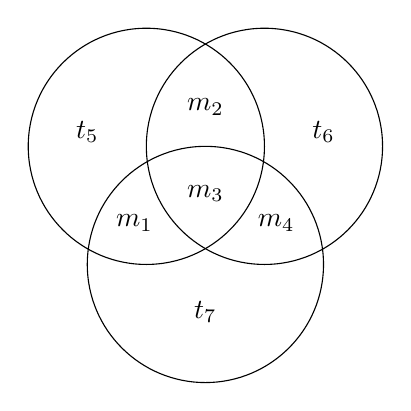
\begin{tikzpicture}
\def\size{1.5}
\def\circleA{(0,0) circle (\size cm)} %top left
\def\circleB{(\size,0) circle (\size cm)} %top right
\def\circleC{(\size/2,-\size) circle (\size cm)} %bottom
\draw\circleA;
\draw\circleB;
\draw\circleC;
\node at (-\size/2,\size/8) {$t_5$};
\node at (\size+\size/2,\size/8) {$t_6$};
\node at (\size/2,\size/3) {$m_2$};
\node at (\size/2,-1.4*\size) {$t_7$};
\node at (-0.1*\size,-0.65*\size) {$m_1$};
\node at (1.1*\size,-0.65*\size) {$m_4$};
\node at (\size/2,-0.4*\size) {$m_3$};
\end{tikzpicture}
\end{center}

For all of the three circles, the parity bit should equal the parity of the three message bits in that circle.

\begin{example}
The decoding of the string 1010100 is performed as follows. First, we fill in the bits into the diagram:
\begin{center}
\begin{tikzpicture}
\def\size{1.5}
\def\circleA{(0,0) circle (\size cm)} %top left
\def\circleB{(\size,0) circle (\size cm)} %top right
\def\circleC{(\size/2,-\size) circle (\size cm)} %bottom
\draw\circleC;
\draw[line width=0.7mm,color=ocre]\circleA;
\draw[line width=0.7mm,color=ocre]\circleB;

\node at (-\size/2,\size/8) {$1$};
\node at (\size+\size/2,\size/8) {$0$};
\node at (\size/2,\size/3) {$0$};
\node at (\size/2,-1.4*\size) {$0$};
\node at (-0.1*\size,-0.65*\size) {$1$};
\node at (1.1*\size,-0.65*\size) {$0$};
\node at (\size/2,-0.4*\size) {$1$};
\end{tikzpicture}
\end{center}
We see that in two of the circles, the parity bit is incorrect. This is called the \term{error syndrome} (for a more formal definition of the error syndrome, see Section~\ref{sec:linear-codes}). By flipping only the bit $m_2$ (which is in the intersection of the top two circles, but not the bottom one), we can fix all the parity bits:
\begin{center}
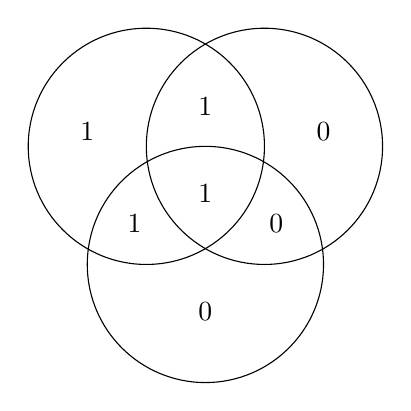
\begin{tikzpicture}
\def\size{1.5}
\def\circleA{(0,0) circle (\size cm)} %top left
\def\circleB{(\size,0) circle (\size cm)} %top right
\def\circleC{(\size/2,-\size) circle (\size cm)} %bottom
\draw\circleC;
\draw\circleA;
\draw\circleB;

\node at (-\size/2,\size/8) {$1$};
\node at (\size+\size/2,\size/8) {$0$};
\node at (\size/2,\size/3) {$1$};
\node at (\size/2,-1.4*\size) {$0$};
\node at (-0.1*\size,-0.65*\size) {$1$};
\node at (1.1*\size,-0.65*\size) {$0$};
\node at (\size/2,-0.4*\size) {$1$};
\end{tikzpicture}
\end{center}
Hence, $\mathtt{dec}(1010100) = 1110$.
\end{example}
The $[7,4]$ Hamming code can correctly decode if the codeword is corrupted in (at most) one place. However, if the codeword is corrupted in two or more places, the Hamming code will not decode correctly. For example, if $\mathtt{enc}(0001) = 0001011$ is corrupted in two places to become 0011010, it will decode to $\mathtt{dec}(0011010) = 0111$. The number of bit flips a code can correct for depends on the minimal distance between the words in the codebook:

\begin{definition}[Hamming distance]
The Hamming distance between two $n$-bit strings $x$ and $y$ is defined as
\[
d(x,y) := \sum_{i=1}^n |x_i - y_i|.
\]
Here, $|z|$ denotes the \term{Hamming weight} of a binary string: the number of ones in that string.
\end{definition}

\begin{definition}[Minimal distance]
Given a code with codebook $C$, the minimal distance of that code is defined as
\[
d_{\min} := \min_{\stackrel{x,y \in C}{x \neq y}} d(x,y).
\]
\end{definition}
By checking all pairs of codewords of the $[7,4]$ Hamming code, one can verify that its minimal distance is 3 (for this reason, it is often called a $[7,4,3]$ code). Hence, if two bits in a codeword are flipped, it might be closer to some other codeword in terms of number of bit flips. By flipping a single bit, the channel output is (incorrectly) decoded into the message that corresponds to that other codeword.

\begin{exercise}
Compute the rate of the $[7,4]$ Hamming code.
\end{exercise}




\subsection{Generalization: linear codes}~\label{sec:linear-codes}
The repetition code and the $[7,4]$ Hamming code both belong to the more general class of linear codes, which we study in this section.

\begin{definition}[Linear code]
A code $C$ is linear if for all $x, y \in C$, also $x + y \in C$.
\end{definition}
In other words, $C$ is linear if it is a subspace of $\mathcal{X}^n$. For the definition of linearity to make sense, addition needs to be defined on $\mathcal{X}^n$. \yfke{or does it even need to be a field?} In the following, we will assume that $\mathcal{X} = \set{0,1}$: in that case addition is simply bitwise addition modulo 2.
\begin{exercise}
Check that the repetition code $R_n$ and the $[7,4]$ Hamming code are indeed linear.
\end{exercise}

For linear codes, the notation ``$[n,k,d]$ (linear) code'' is often used to denote the fact that $n$ bits are used to encode $k$ message bits, with a minimal distance $d$. Be aware that in the notation of Definition~\ref{def:code}, this would be a $(2^k, m)$ code. We use different types of brackets to differentiate between the two notations.

\begin{definition}[Generator matrix]
Given a $[n,k,d]$ linear code, the generator matrix $G^T$ is an $n \times k$ matrix such that the columns $c_1, ..., c_k$ form a basis for $C$. The generator matrix can always be written in \term{systematic form}:
\[
G^T = 
\left(
\begin{array}{c}
\mathbb{I}_k\\
\hline
P
\end{array}
\right),
\]
where $P$ is some $(n-k) \times k$ matrix representing the parity bits of the code.
\end{definition}
The generator matrix is used in the encoding function as follows:
\[
\mathtt{enc}(m) = G^T \cdot m.
\]
The codebook $C$ is the set $\Set{G^T \cdot m}{m \in \mathcal{X}^n}$.

\begin{example}[{Generator matrix of the $[7,4]$ Hamming code}]
The following $7 \times 4$ matrix generates the $[7,4]$ Hamming code:
\[
G^T = 
\left(
\begin{array}{c c c c}
1 & 0 & 0 & 0\\
0 & 1 & 0 & 0\\
0 & 0 & 1 & 0\\
0 & 0 & 0 & 1\\
\hline
1 & 1 & 1 & 0\\
0 & 1 & 1 & 1\\
1 & 0 & 1 & 1
\end{array}
\right).
\]
The generator matrix is given in systematic form. To encode the message 1010, we compute
\[
G^T \left(\begin{array}{c}
1\\0\\1\\0
\end{array}\right) = \left(\begin{array}{c}
1\\0\\1\\0\\0\\1\\0
\end{array}\right).
\]
\end{example}
The decoding operation is specified by the parity-check matrix:

\begin{definition}[Parity-check matrix]
Let $C$ be a code with generator matrix \[G^T = \left(\begin{array}{c}
\mathbb{I}_k\\\hline P
\end{array}\right)\]. Then the parity check matrix for $C$ is given by
\[
H := \left( - P \mid \mathbb{I}_{n-k}\right).
\]
Note that if $\mathcal{X}^n = \{0,1\}^n$, then $P$ is a matrix with binary entries, and hence $-P = P$.
\end{definition}

\begin{definition}[Syndrome]
Let $C$ be a code with parity-check matrix $H$. The syndrome of a received codeword $c \in \mathcal{Y}^n$ is $Hc$.
\end{definition}
For all $c \in C$, the syndrome is the all-zero vector, since $c = G^Tm$ for some $m$, and 
\begin{align}
HG^Tm = \left(-P\mid \mathbb{I}_{n-k}\right)\left(\begin{array}{c} \mathbb{I}_{k} \\\hline P \end{array}\right) m = 0^{n-k}.
\end{align}

The syndrome gives a lot of valuable information about where an error occurred. Suppose a codeword $c$ is sent over a channel, and a single bit of $c$ if flipped, at the $i$th position. The output of the channel is thus $c' = c + e_i$ (where $e_i$ is the $i$th unit vector, which is 1 at position $i$ and 0 elsewhere). The syndrome for this received output is
\begin{align}
Hc' = H(c + e_i) = Hc + He_i = He_i,
\end{align}
which is the $i$th column of $H$. So by comparing the syndrome to the parity-check matrix $H$, we can find out which bit was most likely flipped.

\begin{example}[{Parity-check matrix of the $[7,4]$ Hamming code}]
The following $3 \times 7$ matrix is the parity-check matrix for the $[7,4]$ Hamming code:
\[
H = \left(\begin{array}{c c c c c c c}
1 & 1 & 1 & 0 & 1 & 0 & 0\\
0 & 1 & 1 & 1 & 0 & 1 & 0\\
1 & 0 & 1 & 1 & 0 & 0 & 1\\
\end{array}
\right).
\]
When checking, for example, the codeword 1010100, a syndrome of 110 is observed, which means that the second bit ($m_2$) should be flipped to correct it: the decoding is 1110.
Notice that all columns of $H$ are different, and that there are $2^3 = 8$ possible syndromes we might observe. This aligns well with the fact that there are three parity bits that can all either be correct or incorrect.
\end{example}

\begin{example}[The 5-bit repetition code]
The generating matrix of $R_5$, the 5-bit repetition code, is
\[G^T = \left(\begin{array}{c}
1\\1\\1\\1
\end{array}\right).\]
The parity check matrix is
\[
H = \left(\begin{array}{ccccc}
1&1&0&0&0\\
1&0&1&0&0\\
1&0&0&1&0\\
1&0&0&0&1
\end{array}\right).\]
If the codeword 10100 is received, the syndrome is 1011. This is exactly the vector $e_1 + e_3$, the sum of the first and third column. Hence, we should flip the first and third bit to correct the error. Note that 1011 is also equal to $e_2 + e_4 + e_5$, so another option to arrive at a correct codeword is to flip the second, fourth and fifth bit. It is less likely, however, that three bit flips occurred instead of two.
\end{example}
In general, a code with minimal distance $d$ can \emph{detect} up to $d-1$ bit flip errors, because in $d-1$ bit flip `steps', one can never arrive at another valid codeword. The code can accurately \emph{correct} up to $\frac{d-1}{2}$ bit flip errors. This is because if all codewords are guaranteed to be at least $d$ bit flips apart, the set of strings that result from $\frac{d-1}{2}$ bit flips on a codeword $c_1$ never overlaps with the set of strings that result from that number of bit flips on another codeword $c_2$.

\begin{center}
\def\scale{0.75}
\begin{tikzpicture}

\draw[fill=ocre!50] (0,0) circle (2*\scale);
\draw[fill=black] (0,0) circle (0.5mm);
\node[anchor=north] at (0,0) {$c_1$};

\draw[fill=ocre!50] (5*\scale,1*\scale) circle (2*\scale);
\draw[fill=black] (5*\scale,1*\scale) circle (0.5mm);
\node[anchor=north] at (5*\scale,1*\scale) {$c_2$};

\draw[<->, >=latex] (0,0) -- (5*\scale,1*\scale);
\node at (2.5*\scale,0.7*\scale) {$d$};
\draw[<->, >=latex] (0,0) -- (-1*\scale,1.732*\scale);
\node at (-1*\scale,1*\scale) {$\frac{d-1}{2}$};
\draw[<->, >=latex] (0,0) -- (1*\scale,3.872*\scale);
\node at (1.5*\scale,3*\scale) {${d-1}$};

\draw ({4*cos(215)*\scale},{4*sin(215)*\scale}) arc (215:-35:{4*\scale});

%\begin{scope}
%\clip{(0,0) circle (4*\scale)};
%\draw[fill=black](5*\scale,1*\scale) circle (2*\scale);
%\end{scope}

\end{tikzpicture}
\end{center}
If every codeword needs an area around it that it does not share with any other codeword, this has consequences for the total number of codewords.
\begin{proposition}[Hamming bound]
If $C$ is a \emph{binary} code of block length $n$ and minimum distance 3, then $|C| \leq \frac{2^n}{n+1}$.
\end{proposition}
\begin{proof}
For each $c \in C$, define the neighborhood of $c$ to be $N(c) := \{y \in \{0,1\}^n \mid d(x,y) \leq 1\}$. Every such neighborhood contains exactly $n+1$ elements. Since $d = 3$, $N(c) \cap N(c') = \emptyset$ whenever $c \neq c'$. Hence,
\begin{align}
2^n \geq |\bigcup_{c \in C} N(c)| = \sum_{c \in C} |N(c)| = |C| \cdot (n+1),
\end{align}
and the result follows.
\end{proof}
The $[7,4]$ Hamming code is optimal in the sense that it achieves this Hamming bound: it is a code with block length 7 and minimal distance 3, so an upper bound to the codebook size is $\frac{2^7}{7+1} = 2^4$. The Hamming code achieve exactly this codebook size. There is an entire family of Hamming codes that are optimal in this sense. They form $[2^r-1,2^r-1-r,3]$ codes for $r \in \mathbb{N}$.

We conclude this section with two ways to determine the minimal distance of a code. Apart from the trivial way (determining the entire codebook and comparing all the codeword pairs), it turns out that it is already enough to consider just the Hamming weights of the (nonzero) codewords:


\begin{proposition}
For a code $C$, the minimal distance is equal to the minimal weight of the nonzero codewords.
\end{proposition}
\begin{proof}
The following derivation proves the claim:
\begin{align}
d_{\min} &= \min_{\stackrel{x,y \in C}{x \neq y}} d(x,y) 
= \min_{\stackrel{x,y \in C}{x \neq y}} \sum_{i=1}^n |x_i - y_i| 
= \min_{\stackrel{x,y \in C}{x \neq y}} d(x-y,0)
= \min_{\stackrel{z \in C}{z \neq 0}} d(z,0)
= \min_{\stackrel{z \in C}{z \neq 0}} |z|
\end{align}
\end{proof}

An even faster way to determine the minimal distance of a code is possible if the parity check matrix is known.

\begin{proposition}
For a linear code $C$ with parity check matrix $H$, the minimal distance $d_{\min}$ equals the minimum number of columns of $H$ that are linearly dependent.
\end{proposition}
\begin{proof}
Left as an exercise.
\end{proof}